%!TEX root = ../thesis.tex
%*******************************************************************************
%****************************** Second Chapter *********************************
%*******************************************************************************

\chapter{Theory}
\label{sec:theo}

The theoretical framework of particle physics, the Standard Model (SM), has been developed since the 1960s \cite{GellMann:1961ky,Weinberg:1967tq}.
Up to now it has been successful in explaining most of the observations made in particle physics experiments. 
Especially important for this analysis are predictions concerning top quark production in 
proton-proton collisions, which can be calculated at a high level of accuracy.

In this chapter an overview of the Standard Model is given in Section \ref{sec:theo_sm}. 
The top quark and its properties are explained in Section \ref{sec:theo_top}.
Background processes that are relevant for this measurement of the \ttbar cross section are described in Section \ref{sec:theo_back}.
The simulation used for the \ttbar cross section measurement is described in Section \ref{sec:SimReco_Sim}.


\section{The Standard Model}
\label{sec:theo_sm}

The Standard model is a quantum field theory describing subatomic particles and their interactions.
In the SM there are two types of elementary particles: The fermions with a half integer spin as the fundamental building blocks of matter and 
the bosons with an integer spins as the mediators of the interactions.
It describes the existence of multiple generations of fermions where particles have different masses in each generation, but the same properties otherwise.
After the discovery of the first generation of SM particles (mostly in the first half of the twentieth century), a second and third generation of fermions was discovered by the Stanford Linear Accelerator Center \cite{PhysRevLett.23.935,PhysRevLett.23.930}.
The SM also describes the existence of W and Z bosons, which were then discovered in the 1980s by the UA1 and UA2 experiments at CERN \cite{ARNISON1983103,1983398,BANNER1983476,BAGNAIA1983130}.
These discoveries confirmed the SM the model of particle physics.
The currently known particles of the standard model are shown in Figure \ref{fig:theo_part} with their mass, electric charge and spin.

\begin{figure}[htbp!]
  \begin{center}
      \resizebox{0.65 \textwidth}{!}{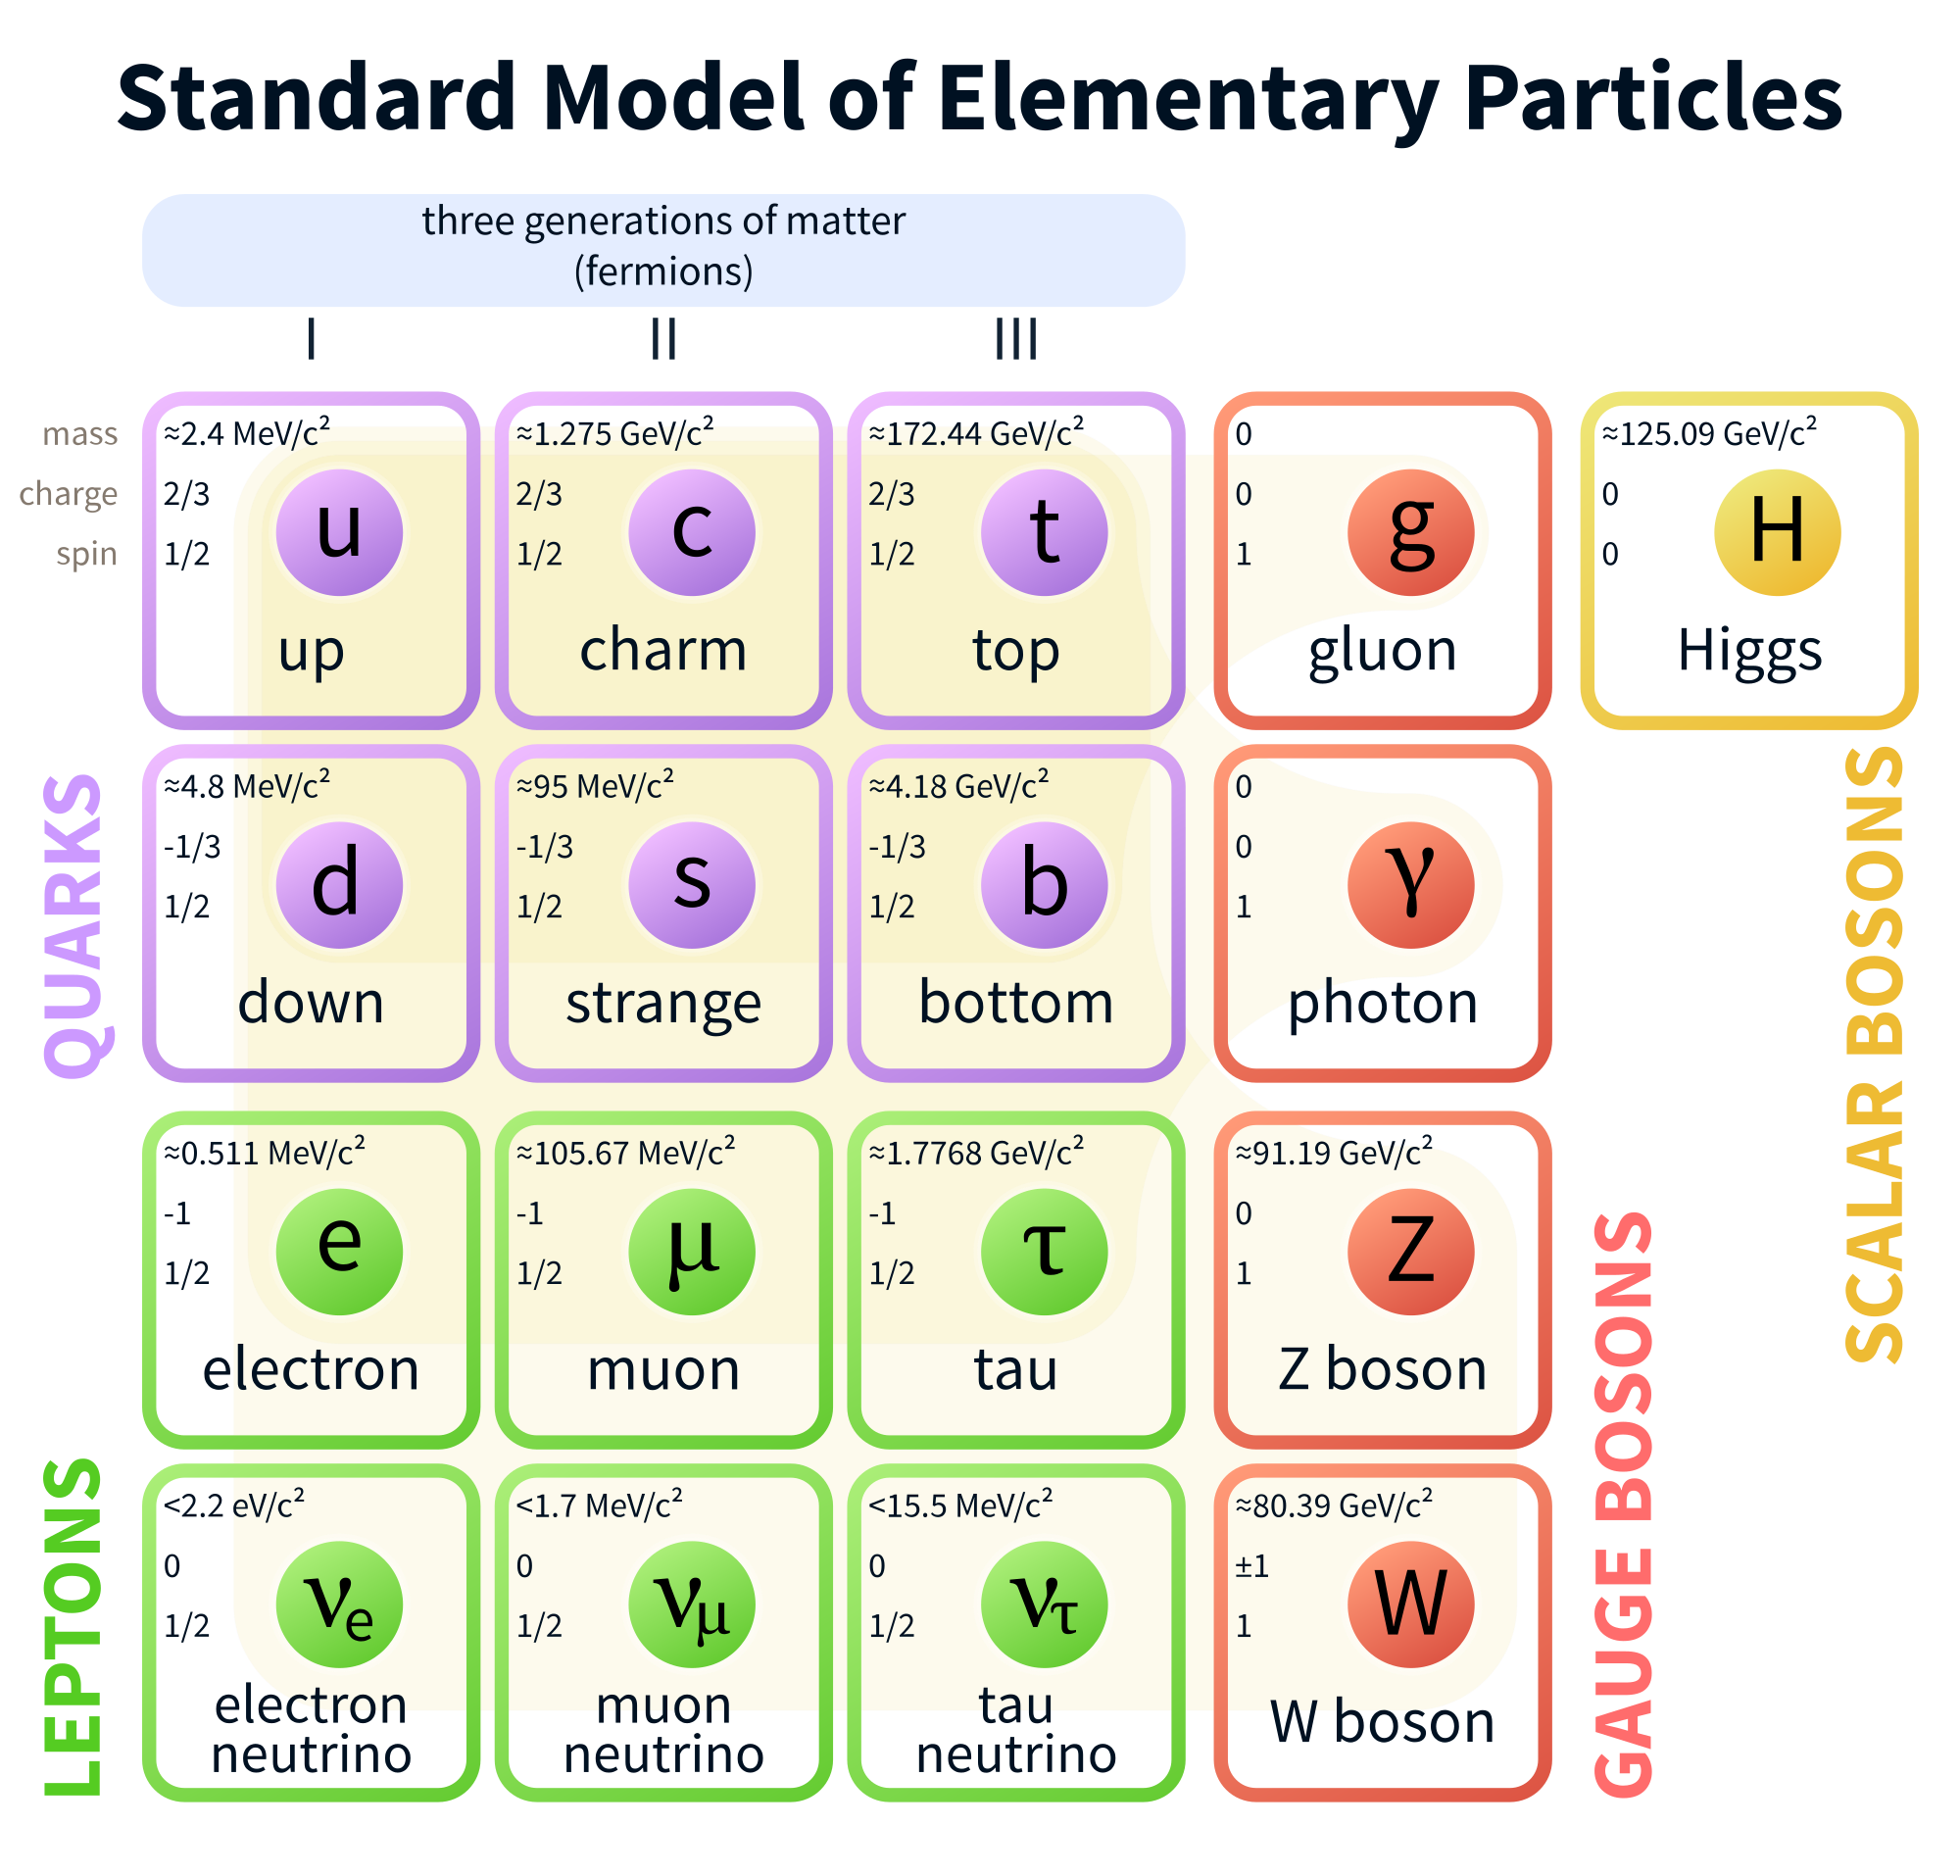
\includegraphics{Theory/Figures/SMPart}}

\caption{The particles of the Standard Model with their respective mass, electric charge and spin \cite{SMPart}. The first three columns show the three generations of fermions. 
The fourth column shows the vector bosons (spin of one). In the right-most column the scalar (spin of zero) Higgs boson is displayed.
  \label{fig:theo_part}}
  \end{center}
\end{figure}


The SM describes three interactions or forces: The strong interaction, the weak interaction and the electromagnetic interaction. The latter two can be unified as  the electroweak interaction.
The strong interaction is mediated by 8 gluons, which carry the charge of the hard interaction, color.
The electroweak interaction is mediated by the photon, the Z boson and the two W bosons. The charge of the electroweak interaction is the weak hypercharge, a combination of the electromagnetic
charge and the weak isospin. Gluons and photons are massless, while the W and Z bosons have a mass, which makes the electroweak interaction 'weak'. These masses are in principle not in line with the  requirement of electroweak symmetry.
The Higgs mechanism \cite{HIGGS1964132,PhysRevLett.13.321,PhysRevLett.13.585} introduces spontaneous breaking of the electroweak symmetry, which allows for massive bosons.
This mechanism also predicted the existence of another boson with zero spin, the Higgs boson, which was discovered in 2012 at the LHC \cite{201230,20121}.

The fermions are further divided into two categories: The leptons which are only affected by the electroweak interaction and the quarks which interact with both the electroweak and the strong force.
There are three generations of fermions, in each generation there are particles with the same properties and a charge difference of one. Only the mass is different, increasing with each generation.

\subsection{The electroweak interaction}
\label{sec:theo_ew}

The unification of the electromagnetic interaction and the weak interaction occurs at the scale of the mass of the bosons mediating the weak interaction (W and Z bosons).
This can be seen in the measurement of deep inelastic electron-proton interactions, which were measured at the highest energies at the HERA collider by the H1 and ZEUS collaborations \cite{Abramowicz:2015mha} (see Figure \ref{fig:theo_ew}). Neutral currents are mediated by the photon and Z boson and charged currents are
mediated by the $\mathrm{W}^+$ and $\mathrm{W}^-$ bosons carrying an electrical charge. The scale where the cross sections of both currents start to agree is the unification scale of the electromagnetic and weak interaction.
Below that scale the weak interaction is suppressed due to the mass of the corresponding bosons.

\begin{figure}[htbp!]
  \begin{center}
      \resizebox{0.75 \textwidth}{!}{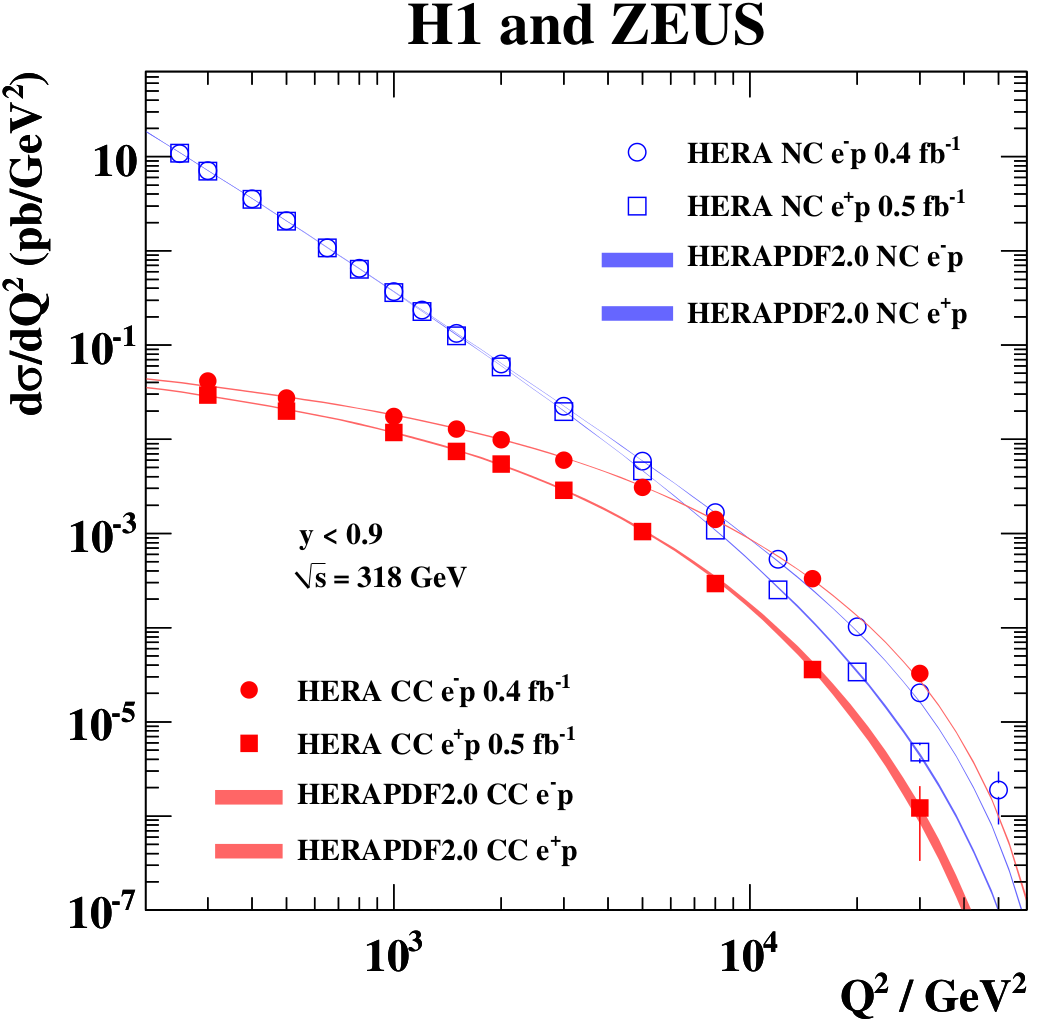
\includegraphics{Theory/Figures/EWUnify}}

\caption{Measurement of the neutral and charged current interaction cross section in $\mathrm{e}^-$p and $\mathrm{e}^+$p collisions by the H1 and ZEUS collaboration \cite{Abramowicz:2015mha}.
The cross sections depend on the total momentum transfer and the measurement is compared to predictions from HERAPDF2.0.
  \label{fig:theo_ew}}
  \end{center}
\end{figure}

The transition or decay of heavier quarks into lighter quarks is explained by the mixing of flavor eigenstates and weak eigenstates. The transition is mediated by a W boson and the 
probability is determined by the Cabibbo-Kobayashi-Maskawa (CKM) matrix. The probability of one quark transitioning to another quark is given by the square of the CKM matrix element $\mathrm{V}_{\mathrm{ab}}$.
The CKM matrix is required to be unitary in the standard model. With that requirement its values are measured to be \cite{Olive:2016xmw}:
 
 \begin{equation}
V_{\mathrm{CKM}}=  
\begin{pmatrix}
\mathrm{V}_{\mathrm{ud}} & \mathrm{V}_{\mathrm{us}} & \mathrm{V}_{\mathrm{ub}} \\
\mathrm{V}_{\mathrm{cd}} & \mathrm{V}_{\mathrm{cs}} & \mathrm{V}_{\mathrm{cb}} \\
\mathrm{V}_{\mathrm{td}} & \mathrm{V}_{\mathrm{ts}} & \mathrm{V}_{\mathrm{tb}} \\
\end{pmatrix}
= 
\begin{pmatrix}
0.947 & 0.225 & 0.004 \\
0.225 & 0.973 & 0.041 \\
0.009 & 0.041 & 0.999 \\
\end{pmatrix}
.
\label{eq:theo_ckm}
\end{equation}

The electroweak interaction is described by a  $\mathrm{SU}(2)_\mathrm{L}\otimes \mathrm{U}(1)_\mathrm{Y}$ gauge symmetry. To preserve that symmetry, all bosons would need to be massless, which contradicts experimental
measurements. 
Particle masses for bosons as well as fermions can be introduced by an additional field, the Higgs field, with a potential that can be written as:

\begin{equation}
V(\Phi) =  \mu^2 \Phi^\dagger \Phi + \lambda(\Phi^\dagger \Phi)^2
\end{equation}
Here, $\lambda$ is restricted to $\lambda > 0$ and $\mu$ to $\mu^2<0$ in order to have non-zero masses. The minima of the potential lead to a non-zero vacuum expectation value of $v = - \mu^2 / \lambda = 246 \; \GeV$\cite{Olive:2016xmw}.
The vacuum expectation value is connected to the masses of the bosons and fermions, but otherwise these masses are free parameters that have to be measured experimentally.

\subsection{The strong interaction}
\label{sec:theo_qcd}

The strong interaction is described by Quantum Chromo Dynamics (QCD), which comprises a $\mathrm{SU}(3)_\mathrm{C}$ gauge group. The charge of the QCD is called color and is mediated by 8 gluons, which are massless bosons.
The interaction length of the strong force is short, due to a phenomenon called confinement. It requires all particles carrying a color charge to form color neutral hadrons, a process called hadronization.

Confinement is caused by the dependence of the coupling of the color charge (strong coupling) $\as$ on the energy scale of an interaction, shown in Figure \ref{fig:theo_as}.

 
\begin{figure}[htbp!]
  \begin{center}
      \resizebox{0.75 \textwidth}{!}{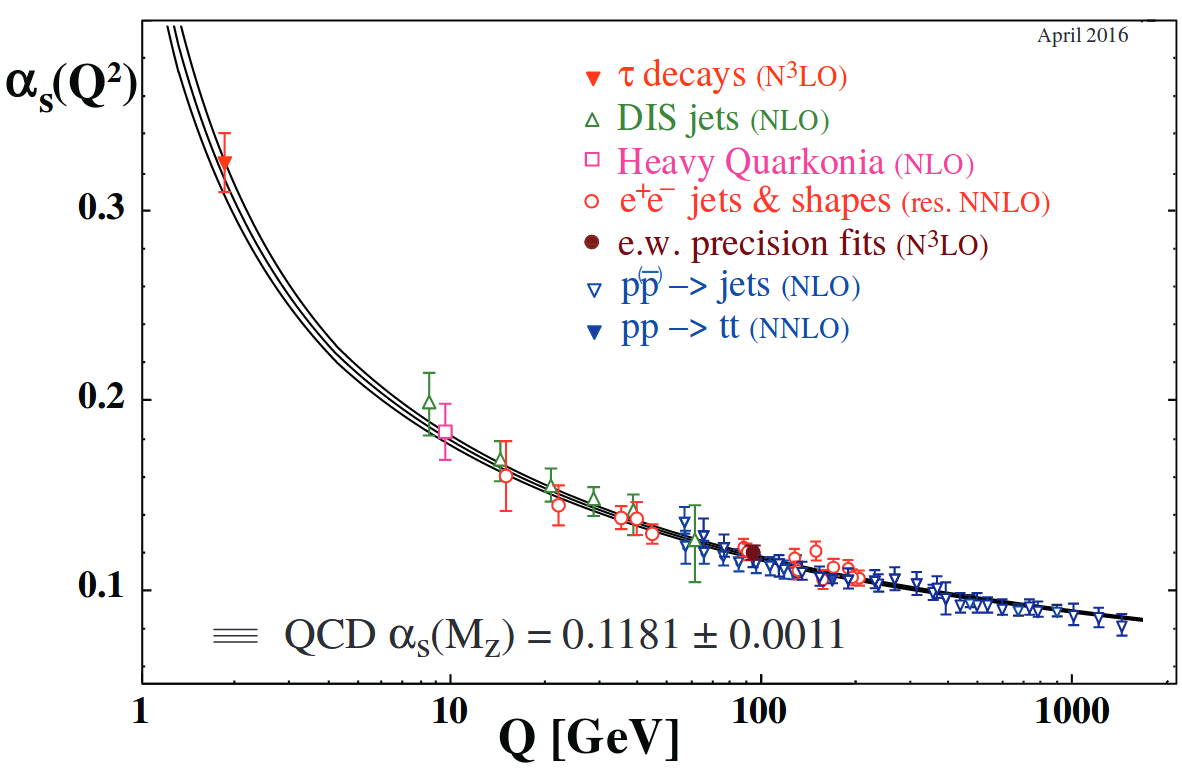
\includegraphics{Theory/Figures/AlphaS}}
\caption{Dependence of \as on the scale $Q^2$ of an interaction \cite{Olive:2016xmw}.
  \label{fig:theo_as}}
  \end{center}
\end{figure}

The strong coupling increases with decreasing momentum transfer. Consequently, the coupling between two quarks increases with larger distances. This makes it energetically more beneficial to create a new quark anti-quark pair.
This means that no bare color charge can exist for an extended period of time; the color is confined. The quarks, together with gluons, eventually form bound states, which are required to be colorless and are called hadrons. 
For the three colors (red, green and blue) a color neutral hadron can contain three valence quarks with a different color each and be called a baryon. Hadrons can also be formed from two quarks which have to form a pair of color
and anti color (quark and anti quark). These hadrons are called mesons. Beside the proton all hadrons are unstable and decay eventually.
The process of the creations of these hadrons 
is called hadronization. A single high energetic quark will produce multiple hadrons which are collimated due to the momentum of the initial quark. In a detector, these collimated hadrons are measured as a so-called jet. 

For high energies or short interaction scales the coupling strength decreases. This effect is called asymptotic freedom. It allows the quarks in a bound state, for example inside the proton, to be treated as free.
At high scales the interaction can be calculated perturbatively, while processes at low scales such as hadronization are usually calculated based on phenomenological models.


\section{The top quark}
\label{sec:theo_top}

The top quark is the heaviest particle in the Standard Model and the heaviest elementary particle known today. It was discovered in 1995 by the \DZERO and CDF collaborations at the Tevatron \cite{PhysRevLett.74.2626,PhysRevLett.74.2632}. Due to its high mass, it decays before hadronization, which allows to measure properties of the bare quark through the decay products. Multiple theories that extend the Standard Model predict particles that decay into top quarks. An example would be a massive \zp boson in extended gauge theories \cite{PhysRevD.63.035006,ROSNER1996113} decaying into a \ttbar pair. A supersymmetric top partner stop or top squark could also decay into a top quark and a neutralino, leading
to a process very similar to \ttbar production \cite{NILLES19841,FARRAR1978575}. Anomalous top quark couplings could also affect the production of top quarks as well as their decay \cite{PhysRevD.91.114010,PhysRevD.82.114008,PhysRevD.80.114017}.

\subsection{Top quark pair production and decay}
\label{sec:theo_prod}

The calculation of top quark pair production at the LHC can be factorized into a high energy ('hard') scattering process and the distribution of the momenta of the initial partons.
At the LHC the probability to find a quark or gluon of a certain energy in the initial state is given by Parton Density Functions (PDFs), which can be measured independently from a specific physics process.
The cross section can then be calculated perturbatively according to \cite{Husemann:2017eka}: 

\begin{equation}
\sigma = \sum_{jk}^{partons} \int_0^1 \mathrm{d}x_k\mathrm{d}x_j f_j(x_j,\muf) f_k(x_k,\muf) \hat{\sigma}(x_j,x_k,s,\muf,\as(\mur))
\end{equation}

The PDFs $f_i(x_i,\muf)$ give the probability to find a parton $i$ with the momentum fraction $x_i$ in the initial state when the initial state hadron is probed at the scale $\muf$. The factorization scale $\muf$ separates
the hard process from the PDF, which absorbs infrared or collinear divergencies in the initial state. The scattering amplitude or hard cross section $\hat{\sigma}$ depends on the momentum fraction of the partons, the squared 
center of mass energy $s$ and the strong coupling constant \as calculated at defined scale $\mur$. Introducing the renormalization scale $\mur$ as a cut-off avoids ultraviolet divergencies in virtual corrections of the production cross section.

For proton-proton collisions at a center of mass energy of $\sqrt{s}=13\;\TeV$, top quark pairs are mainly produced by gluon-gluon fusion. Only about $10\%$ of \ttbar pairs
are produced through quark anti-quark annihilation \cite{Olive:2016xmw}. The production via gluon-gluon fusion can occur in the s-, t- or u-channel. Feynman graphs for these production processes
are shown in Figure \ref{fig:theo_ttfeyn}.

\begin{figure}[htbp!]
  \begin{center}
      \resizebox{0.75 \textwidth}{!}{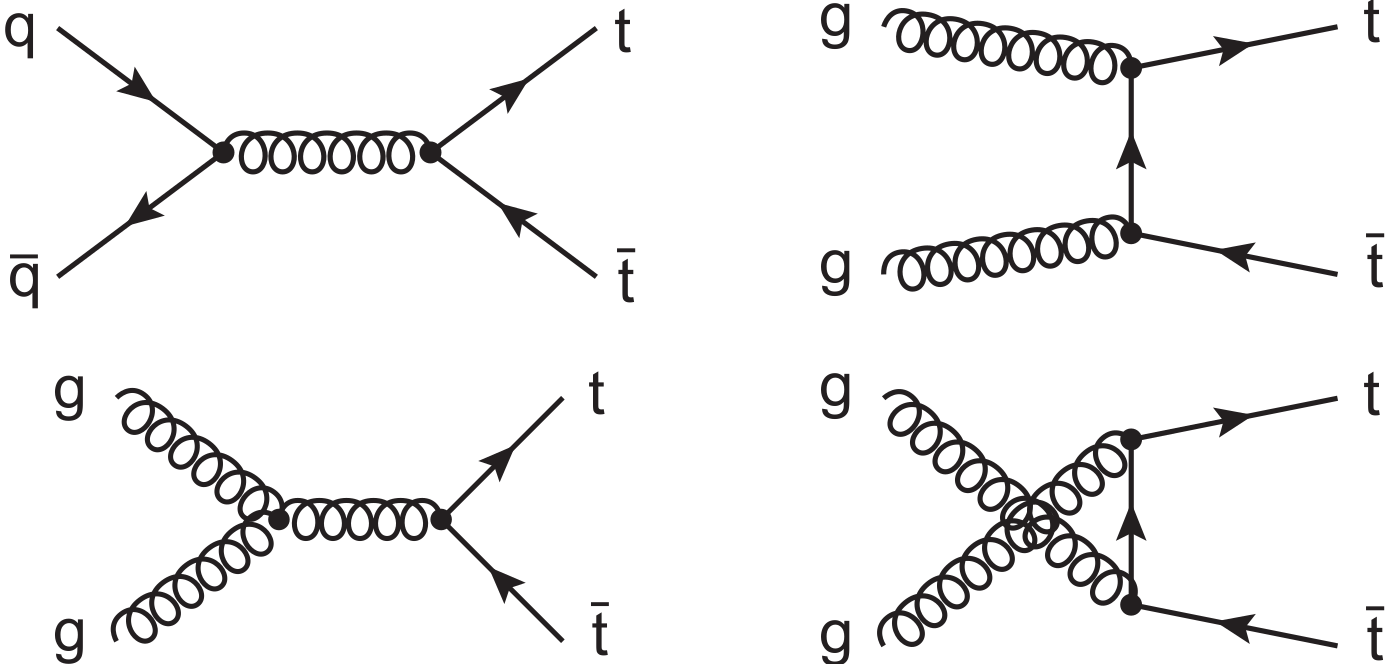
\includegraphics{Theory/Figures/ttbar_feyn}}
\caption{Feynman graphs for \ttbar production from gluon-gluon fusion and quark antiquark annihilation (upper left) \cite{Husemann:2017eka}. The production from gluon-gluon fusion is shown in the s- (lower left),t- (upper right) and u-channel (lower right).
  \label{fig:theo_ttfeyn}}
  \end{center}
\end{figure}

Proton-proton collisions can also result in the production of single top quarks via the electroweak interaction. 
The single top quark production can occur in the t- and s-channel or with an associated W boson. Respective Feynman diagrams are shown in Figure \ref{fig:theo_stfeyn}.

\begin{figure}[htbp!]
  \begin{center}
      \resizebox{0.25 \textwidth}{!}{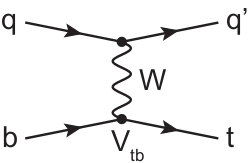
\includegraphics{Theory/Figures/ST_tch}}
      \resizebox{0.25 \textwidth}{!}{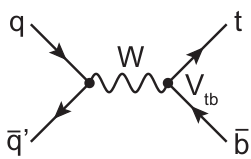
\includegraphics{Theory/Figures/ST_sch}}
      \resizebox{0.25 \textwidth}{!}{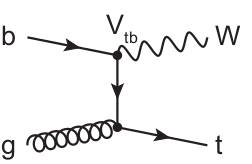
\includegraphics{Theory/Figures/ST_tW}}
\caption{Feynman graphs for single top quark production in the t- (left), s-channel (middle) and with an associated W boson (right) \cite{Husemann:2017eka}. 
  \label{fig:theo_stfeyn}}
  \end{center}
\end{figure}

Due to its high mass, the top quark has a very short lifetime. It decays before it would hadronize.
Top quarks almost exclusively decay into a W boson and a b quark, due to the high value of the CKM matrix element $\mathrm{V}_{\mathrm{tb}} = 0.999$ (see Equation \ref{eq:theo_ckm}).
A \ttbar pair consequently decays into two W bosons and two b quarks. At next-to-leading order (NLO) of QCD the $\mathrm{gg} \rightarrow \mathrm{WbWb}$ process also enters into calculations of single top production with an 
associated W boson leading to interference with \ttbar production \cite{Cascioli:2013wga}. The two processes can still be treated separately \cite{White:2009yt}.

The total production cross section at a center of mass energy of $\sqrt{s}=13\;\TeV$ has been calculated at NNLO+NNLL as \cite{Czakon:2013goa}:

\begin{equation}
\sigma_{\ttbar}   =   \xsectheo. 
\end{equation}

This very precise calculation can be tested by an equally precise measurement. Besides probing higher order QCD calculations, the comparison of the measured and predicted cross section can also be used to constrain
anomalous phenomena. It can also be used to determine other SM parameters like the strong coupling constant \as.

The cross sections for several processes in proton-proton collisions are shown in Figure \ref{fig:theo_xsecs}. The \ttbar production cross section increases significantly with the center of mass energy, especially compared to other 
processes.
Nevertheless, the cross section for the production of b quarks and W or Z bosons is significantly higher at a center of mass energy of $\sqrt{s}=13\TeV$. The ability to distinguish \ttbar events from these other processes depends on 
the decay products of the top quarks.


\begin{figure}[htbp!]
  \begin{center}
      \resizebox{0.5 \textwidth}{!}{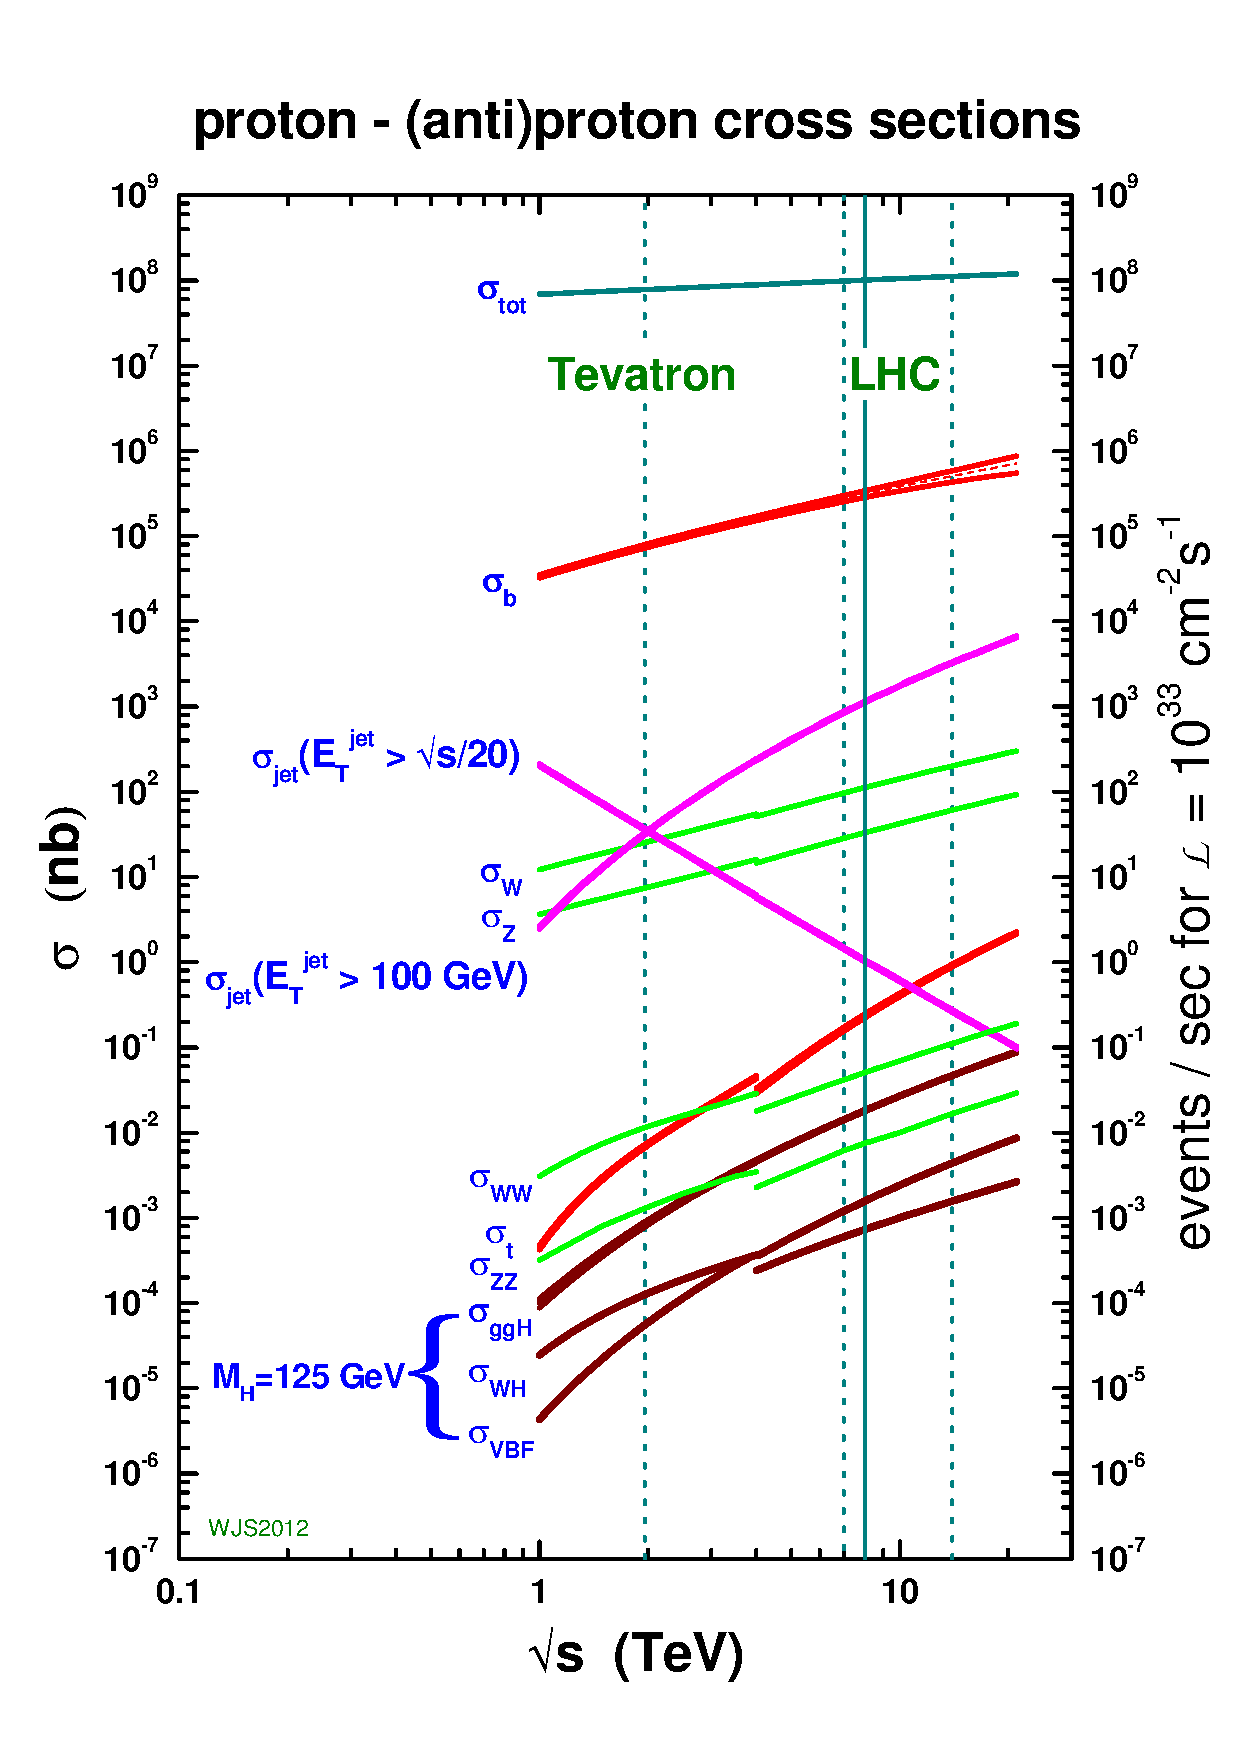
\includegraphics{Theory/Figures/Xsecs}}
\caption{Cross sections for several processes at the Tevatron and the LHC depending on the center of mass energy $\sqrt{s}$\cite{Olive:2016xmw}.
  \label{fig:theo_xsecs}}
  \end{center}
\end{figure}


After the decay of the top quark into a W boson and a b quark, the W boson further decays into a lepton and the associated neutrino or into two quarks.
Decays of \ttbar events are separated into decay channels according to the decay of the W bosons.

In the all-hadronic decay channel, both W bosons decay into quarks: $\mathrm{tt} \rightarrow \mathrm{q}\overline{\mathrm{q}}b \; \mathrm{q}\overline{\mathrm{q}}\overline{\mathrm{b}}$. This channel has the highest branching ratio of $\sim 45\%$, but it suffers from a lot of background contamination,
since the cross section to produce multiple jets in proton-proton collisions is large compared to the \ttbar cross section. This makes the all-hadronic channel unsuitable for a high precision measurement of the \ttbar cross section.

In the semileptonic decay channel one W boson decays into quarks, the other into leptons: $\mathrm{tt} \rightarrow \mathrm{l}^+ \nu_l b \; \mathrm{q}\overline{\mathrm{q}}\overline{\mathrm{b}}$. This channel has a similar branching ratio to that of the all-hadronic channel at $45\%$, including events with $\tau$ leptons. 
The lepton in the final state makes the events easier to distinguish from background events. However, the cross section for W+jets production is still significantly higher, leading to a sizable background contamination.

In the dilepton decay channel both W bosons decay into leptons: $\mathrm{tt} \rightarrow \mathrm{l}^+ \nu_l b \; \mathrm{l}^- \overline{\nu_\mathrm{l}}\overline{\mathrm{b}}$. This channel has a comparatively low branching ratio of $\sim 10\%$, including $\tau$ leptons. The decays of $\tau$ leptons into quarks again effectively reduce the branching ratio.
The dilepton decay channel has a clear signature thanks to the two leptons in the final state. The largest source of background events is Drell-Yan (Z+jets) process, which has a higher production cross section than the \ttbar process, but can be distinguished by the Z mass peak in the dilepton mass spectrum.
Especially the \emu decay channel combines a clear signature with a low background: Muons leave a clear signature in the detector and the main background from Drell-Yan events is reduced by requiring opposite flavored leptons in the final state.

The dilepton decay channel is suitable to achieve the highest possible precision for the measurement of the \ttbar cross section.

\subsection{The top quark mass}

The top quark mass is defined by its Yukawa coupling to the Higgs field. Conversely, since the mass is large, the Yukawa coupling is predicted to be large compared to the coupling of lighter particles.
In both measurements and theory calculations, the top quark mass can be determined in multiple ways.

In a direct measurement of the top quark mass the decay products are identified and the invariant mass distribution of the decay products is measured. The relation of the observed to the actual top quark mass is usually provided by Monte Carlo (MC) generators.
This method allows measuring the top quark mass with a high experimental precision \cite{ATLAS:2014wva,Khachatryan:2015hba}. Since the simulation of \ttbar decays includes phenomenological models
the mass measured in such measurements does not exactly correspond to the mass definition used in theoretically well-defined calculations.

Perturbative calculations often use the pole mass definition, \mtp. It is well defined in every order of perturbation theory \cite{Bigi:1994em}, but it suffers from non-perturbative ambiguities \cite{Dowling:2013baa,Beneke:1994sw}.
It has been shown that this so-called renormalon ambiguity is of the size of $70\; \MeV$ \cite{Beneke:2016cbu}.
It can be measured indirectly by measuring other top quark parameters and comparing them to theory predictions depending on \mtp. The predicted top quark pair production cross section depends on the assumed pole mass and can be
used to extract the pole mass \cite{Aad:2014kva,Khachatryan:2016mqs}. The precision of these measurements is not only limited by the uncertainties on the measurement, but also by the theoretical uncertainties on \mtp.
The top quark mass implemented in MC generators is assumed to be close to the pole mass \cite{Buckley:2011ms}, but a uncertainty of up to $1\;\GeV$ remains.

The scale-dependent top quark mass in the \msbar scheme does not contain non-perturbative ambiguities. It has also been shown to converge faster than the pole mass \cite{Dowling:2013baa}, leading to generally lower theoretical
uncertainties. The relation to the pole mass is known to a high precision \cite{Marquard:2015qpa}. Similarl to the pole mass it can be extracted from measurements of top quark parameters like the \ttbar cross section \cite{Abazov:2011pta}. 

The top quark mass is an important parameter in electroweak fits that are used to probe the SM prediction on the relation of several electroweak parameters \cite{Baak:2014ora}.
The SM can be extrapolated to the Planck scale. In this extrapolation the Higgs vacuum state has implications on the stability of the universe \cite{Buttazzo:2013uya}.
The stability of the vacuum state strongly depends on the Higgs mass, the top mass and \as. In Figure \ref{fig:theo_stability} the stability is shown depending on the 
Higgs and the top mass. The current values for these masses hint at a metastable vacuum. Slightly different parameters could however lead to either a stable vacuum or contradictions
to the observed lifetime of the universe.

\begin{figure}[htbp!]
  \begin{center}
      \resizebox{0.75 \textwidth}{!}{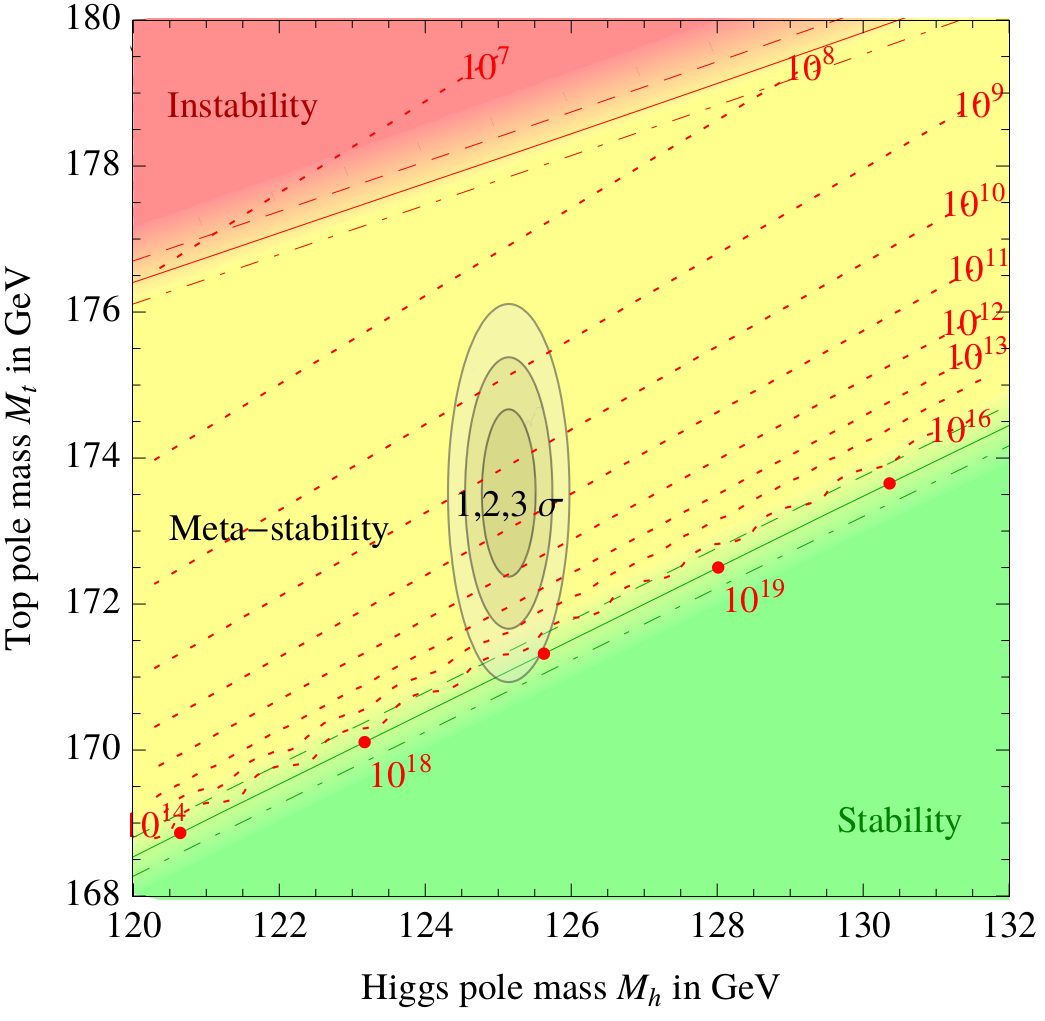
\includegraphics{Theory/Figures/Stability}}
\caption{SM phase diagram depending on the mass of the top quark and the Higgs boson \cite{Buttazzo:2013uya}. The boundary lines denote the uncertainty on the coupling $\as(\mathrm{M}_Z)=0.1184\pm0.0007$
  \label{fig:theo_stability}}
  \end{center}
\end{figure}

\section{Background processes}
\label{sec:theo_back}

In an experiment, top quarks are not measured directly, but they are identified by their decay products. In the dilepton channel, which is used in this analysis, the \ttbar decay produces the following final state:
$\mathrm{tt} \rightarrow \mathrm{l}^+ \nu_l b \; \mathrm{l}^- \overline{\nu_\mathrm{l}}\overline{\mathrm{b}}$.
The two neutrinos cannot be detected, so the signature in the detector consists of two leptons (electrons or muons) and two b quarks, which result in jets.
For this analysis events are mainly selected according to the leptons.
Multiple different SM processes can lead to a similar or even the same signature. The impact of these background events is an important part of the \ttbar cross section measurements and the underlying physics processes are shortly described below.

The largest source of background events in the dilepton channel is the  Drell-Yan \cite{CarloniCalame:2007cd} process. A Z boson is produced through electroweak interaction and decays into two leptons. Two b quarks can originate from initial state radiation, which leads to the
same final state measured for \ttbar events. In the \emu channel Drell-Yan events suppressed, since the Z boson cannot directly decay into opposite flavor leptons.
The total cross section for the $\mathrm{pp}\rightarrow\gamma^{\star}/\mathrm{Z}\rightarrow \mathrm{e}^+\mathrm{e}^- / \mu^+ \mu^-$ process is calculated to be $\sigma_{\mathrm{DY}}= 28.6 \si{\femto \barn}$ for 
$m_{\mathrm{ll}} < 10 \; \GeV$ at NNLO with FEWZ 3.1 \cite{Gavin:2010az}.

Events with W bosons are produced via the electroweak interaction, similar to Drell-Yan events \cite{PhysRevD.86.034021}. In this case the W boson decays into a lepton and a neutrino and two b quarks can be the result of
initial state radiation. Since there is only one lepton in the final state, the contribution of W+jets events is strongly suppressed in the dilepton channel. An additional jet can be reconstructed as a lepton, but this happens rarely.
The cross section for $\mathrm{pp}\rightarrow\mathrm{W}\rightarrow \mathrm{l}\nu_{\mathrm{l}}$ is calculated to be $\sigma_\Wjets=61\si{\femto \barn}$ at NNLO with FEWZ 3.1 \cite{Gavin:2010az}.

Events where two bosons are produced (WW,WZ and ZZ events)\cite{doi:10.1146/annurev-nucl-102010-130106} are another background for \ttbar events in the dilepton channel . They can easily have 2 leptons in the final state, depending on the decay. These events can also contribute in the opposite flavor channel, especially when both bosons decay into leptons.
The cross sections for WZ and ZZ production are calculated at NLO with MCFM \cite{Campbell:1999ah,Campbell:2011bn} to be $\sigma_{\mathrm{WZ}}=45\pb$ and  $\sigma_{\mathrm{ZZ}}=15\pb$.
The cross section for WW productions is calculated at NNLO to be $\sigma_{\mathrm{WW}}=119\pb$\cite{Gehrmann:2014fva}.

Single top production with an associated W boson can result in a final state that has the same signature as the \ttbar signal process (see Section \ref{sec:theo_prod}). The process is hard to distinguish from the \ttbar signal experimentally, but its cross section is small compared to the signal cross section. 
The cross section is calculated at NLO and NNLL to be $\sigma_{\mathrm{tW}}= 71.2\pb$ \cite{bib:twchan}.




\section{simulation}
\label{sec:SimReco_Sim}

The simulation of events involves multiple algorithms, most of which are shown in Figure \ref{fig:sim_struct}

\begin{figure}[htbp!]
  \begin{center}
      \resizebox{0.49 \textwidth}{!}{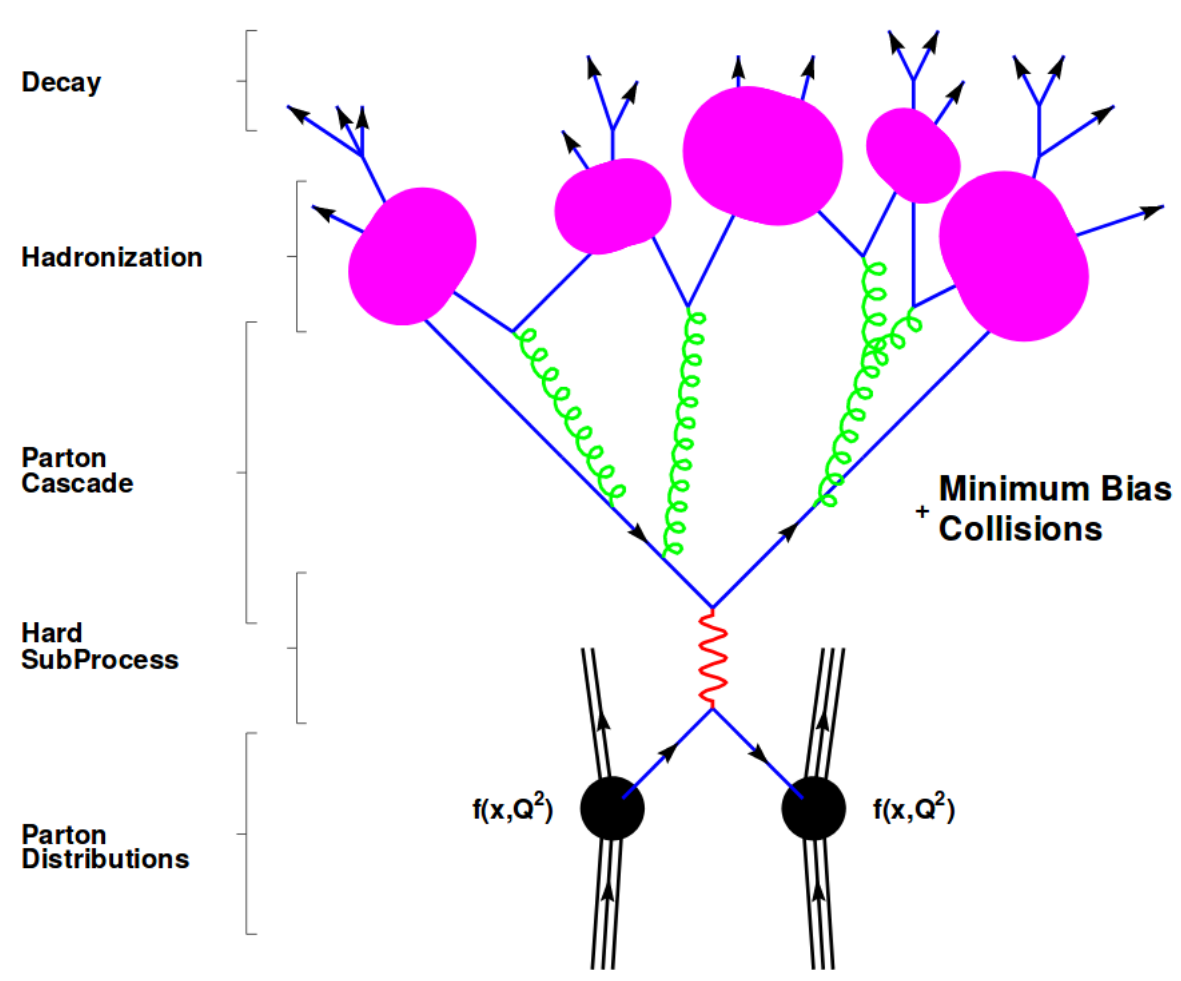
\includegraphics{SimReco/Figures/Event}}
\caption{Illustration of a simulated event split in multiple steps. Starting from the protons and the PDF continuing with the hard interaction, the parton shower, the hadronization and the decay of the hadrons\cite{Dobbs:684090}.
  \label{fig:sim_struct}}
  \end{center}
\end{figure}

The hard interaction for a given process like the production of \ttbar in proton-proton collisions is simulated by the matrix element generator.
This algorithm calculates the scattering amplitude of a given process and the kinematic properties of the resulting partons.
A large number of events is needed to avoid any bias due to the probabilistic nature of these distributions.
The interaction itself is calculated at a fixed order of QCD and can include additional radiation of quarks or gluons from the initial as well as the final state.
In the case of \ttbar events, the matrix element generator also calculates the decay of the top quarks and the W bosons including the impact of spin correlations.

Since the particles in the initial state of the hard process are the constituents of the proton, the probability to find a given constituent in a proton with a certain fraction of energy needs to be known.
This probability is given by Parton Distribution Functions (PDF) that predict the energy fraction of a given quark or gluon that is part of the proton.
In order to avoid singularities in the PDF calculation as well as in the hard interaction, scales for the calculations of these divergences are introduced.
For the calculation of the proton substructure the factorization $\mu_F$ is used, while the scattering amplitude calculation uses the renormalization scale $\mu_R$.
The value of these scales is normally motivated by the mass of the heaviest particle involved in the process.

Radiation beyond the scale of the matrix element generator is simulated by parton shower algorithms.
The radiation is calculated at a scale that can be set separately for initial and final state radiation. 
The parton shower algorithms generally follow phenomenological models and principally include QCD calculations up to all orders.
However, the parameters of these models are commonly tuned to match data from previous measurements.

As indicated by the name, the parton shower also simulates the showering of the partons that are the result of the hard process.
Especially quarks and gluons carrying a color charge contribute to further radiation forming hadronic showers.
These parton showers start from a maximum scale and evolve until a minimum scale on the order of \GeV. 

The combination of radiation of matrix element generator and parton shower can lead to double counting of radiation when the phase space overlaps.
This double counting can be minimized by using a matching procedure which varies according to the generator of parton shower that is used.

After the parton shower is cut off by the scale, the resulting parton showers form color neutral hadrons.
This process is called hadronization and is part of the parton shower algorithm.
Again the hadronization is based on phenomenological methods the settings of which have to be tuned.

The proton constituents not involved in the hard interaction are called proton remnants. The interaction of these proton remnants usually involve low energy processes and form the underlying
event (UE). The UE modelling is again tuned to data and included in the Parton Shower algorithm.

\begin{figure}[htbp!]
  \begin{center}
      \resizebox{0.49 \textwidth}{!}{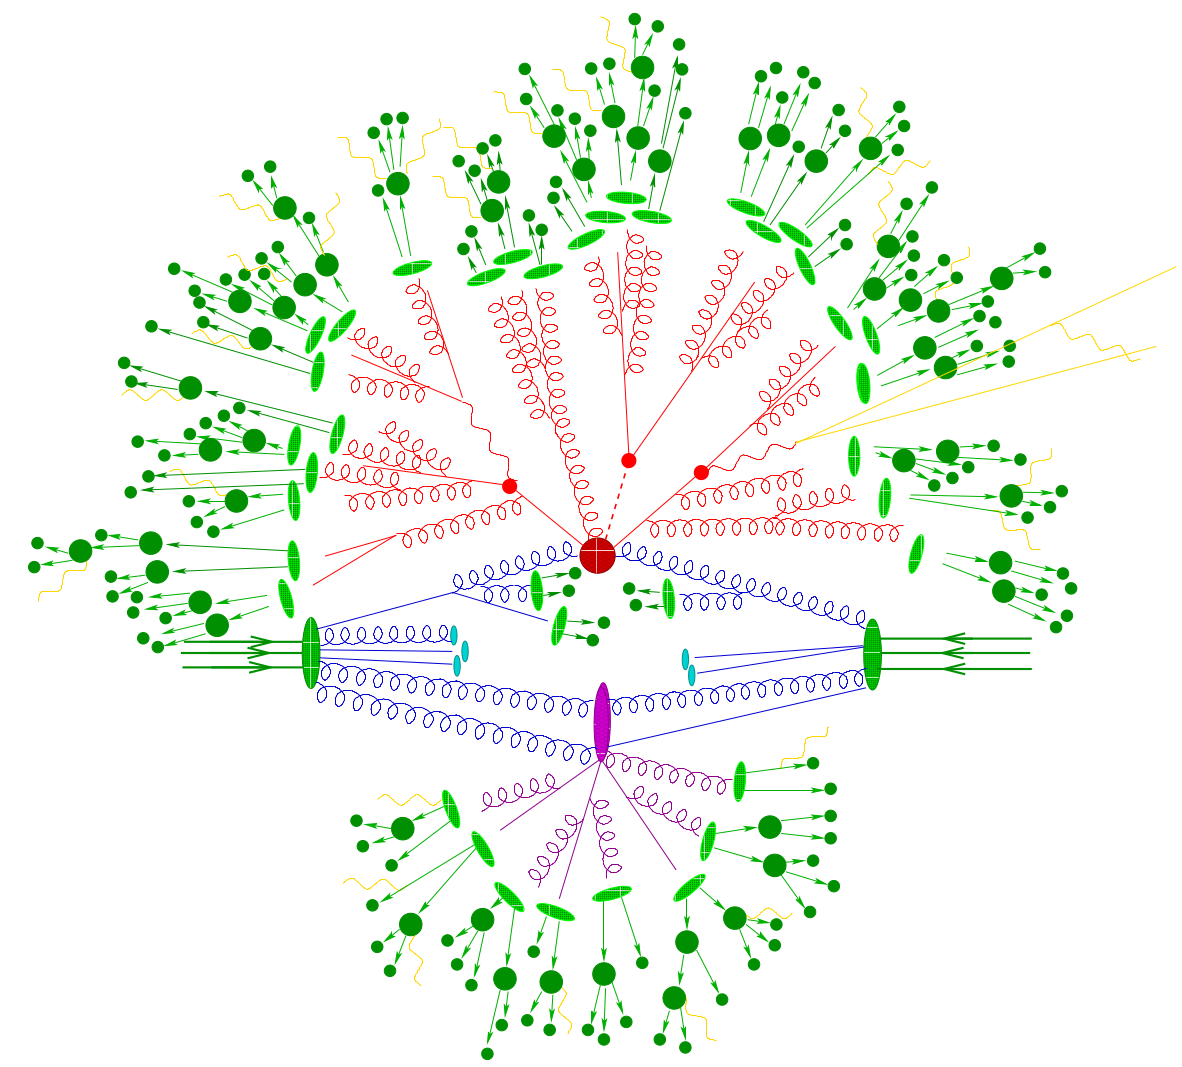
\includegraphics{SimReco/Figures/Sherpa}}
\caption{Representation of a simulated event from the Sherpa generator. It includes the hard interaction as well as showering, hadronization and underlying event\cite{Gleisberg:2008ta}.
  \label{fig:sim_sherpa}}
  \end{center}
\end{figure}

A whole event including the hard process and the parton shower is illustrated in Figure \ref{fig:sim_sherpa} showing the production of a top quark pair in association with a Higgs boson.
The incoming protons on the left and right sides are shown in the middle, with the blue gluons representing the initial state of the hard interaction.
The large red circle stands for the hard interaction, with the initial state radiation shown in blue below.
The partons resulting from the hard interactions are shown above the hard process with smaller red circles. The final state radiation of gluons is also shown in red, while additional radiation of photons is shown in orange.
The partons from the parton shower hadronize as illustrated by the green ellipses. The hadrons then decay into further hadrons.
Below the whole interaction, the underlying event is shown in violet.

The last part of the simulation is the modelling of the detector response which includes modelling the complete detector, simulating the interaction of particles with the detector material and the corresponding
response of the detector electronics. The full response of all detector subsystems including the trigger system is modelled for each event.

In this analysis the main generator is \Powheg~(v.~2)~\cite{bib:powheg2,Frixione:2007vw,Nason:2004rx}, which calculates the relevant process at NLO. 
It is used for the simulation of the \ttbar signal \cite{Frixione:2007nw} as well as for the tW \cite{Re:2010bp} and the Drell-Yan \cite{Kardos:2014dua,Alioli:2010qp} background process.
The W+jets process is generated using \MGaMCatNLO~2.2.2~\cite{Alwall:2014hca,Frederix:2012ps} at NLO including up to two additional jets. The diboson background samples are generated with \Pythia~8.2~\cite{Sjostrand:2014zea}.
All samples are simulated with the NNPDF3.0~\cite{Ball:2012cx} PDF set.

\Pythia~8.2 is also used as parton shower algorithm for all samples. The CUETP8M2T4 tune~\cite{CMS-PAS-TOP-16-021,Skands:2014pea} is used for the simulation of the signal and the tW and Drell-Yan backgrounds.
The tuning is optimized for top physics by including \ttbar data taken with the CMS detector at a center of mass energy of $8 \TeV$.
For the remaining backgrounds, the standard tune for CMS CUETP8M1 tune is used.
\GEANT4 \cite{geant} is used to simulate the detector response for all samples.

The relevant cross sections for the relevant processes are taken from specific theory calculations as described in Section \ref{sec:theo_back}.



